\section{Modular Architecture}
%TODO: this section is a stub
Reprotool project can be seen as a collection of Eclipse plugins built upon Eclipse platform distributed together as a standalone \ac{RCP} application.
List of plugins is presented in Appendix~\ref{sec:plugins}.

%Something about modularization of the application using OSGi.
Eclipse platform uses Equinox implementation of the OSGi. OSGi is a specification defining module system and service platform for the Java programming language.

%What are the benefits of using OSGi instead of plain Java.
In contrast to using plain Java \verb|.jar| libraries OSGi bundles allow to specify required bundles and it's versions. They also allow developer to specify exported packages visible for use from other bundles providing better encapsulation for non-exported ones.

%Eclipse plug-ins and a summary of used concepts.
%Image of the Eclipse platform architecture (something like \url{http://www.webcollab.com/alee/papers/avios05-docbook/pics/eclipse-platform.gif})
	


\subsection{Reprotool Architecture Overview}
%TODO: this section is a stub
Overview of reprotool modules/plugins, see Figure~\ref{fig:ArchitectureOverview}
	
\begin{figure}[ht]
  \centering
  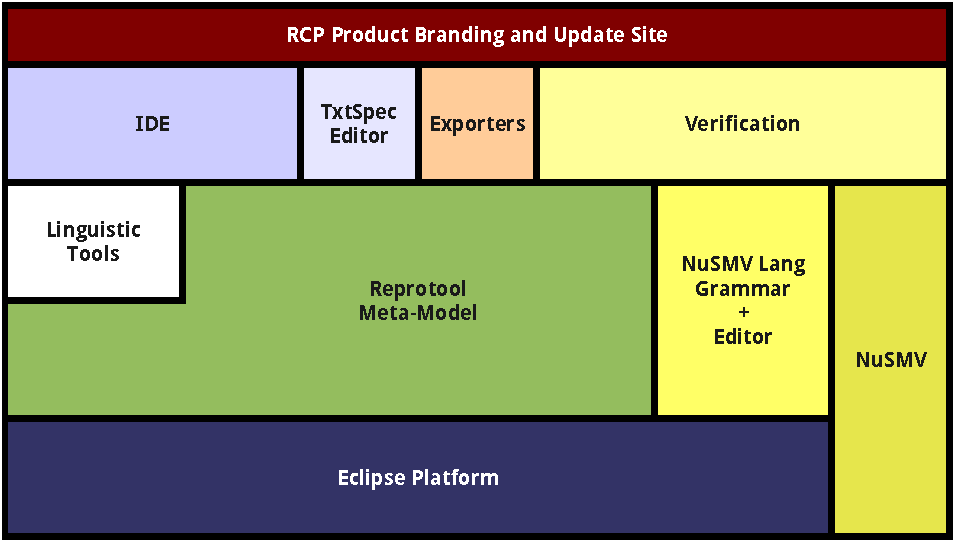
\includegraphics[width=\textwidth]{images/ArchitectureOverview}
  \caption{Reprotool Architecture Overview}
  \label{fig:ArchitectureOverview}
\end{figure}

